% inkscape cantor.pdf --export-type=png --export-filename=cantor.png --export-width=1024 --export-background-opacity=0
% \documentclass[a3paper]{article}
% \usepackage[left=0mm,top=1cm,right=0mm,bottom=0mm]{geometry}
\documentclass[border=0]{standalone}
% \documentclass[dvisvgm]{minimal}
\usepackage{tikz}
\usetikzlibrary{calc,lindenmayersystems}
\usepackage{xcolor}
\definecolor{pGreen}{HTML}{663366}
\definecolor{pRed}{HTML}{336633}
\pgfdeclarelindenmayersystem{Cantor set}{
    \rule{F -> FfF}
    \rule{f -> fff}
}
\begin{document}
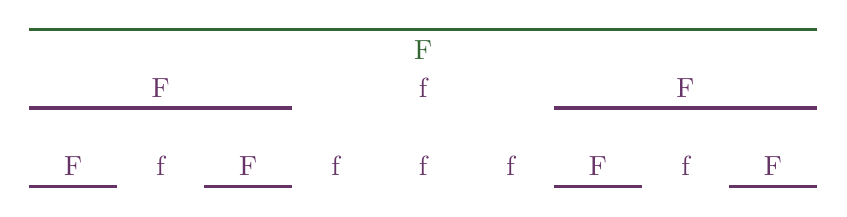
\begin{tikzpicture}
      \coordinate (F) at (0,0)++(0:10);
      \draw[very thick, pGreen] (0,0) -- node[midway,above] {F} (0:10/3);
      \draw[very thick, white] (0:10/3) -- node[midway,above,pGreen] {f} (0:20/3);
      \draw[very thick, pGreen] (0:20/3) -- node[midway,above] {F} (0:10);

      \draw[very thick, pGreen,yshift=-1cm] (0,0) -- node[midway,above] {F} (0:10/9);
      \draw[very thick,yshift=-1cm,white] (0:10/9) -- node[midway,above,pGreen] {f} (0:20/9);
      \draw[very thick, pGreen,yshift=-1cm] (0:20/9) -- node[midway,above] {F} (0:10/3);
      
      \draw[very thick,yshift=-1cm,white] (0:10/3) -- node[midway,above,pGreen] {f} (0:40/9);
      \draw[very thick,yshift=-1cm,white] (0:40/9) -- node[midway,above,pGreen] {f} (0:50/9);
      \draw[very thick,yshift=-1cm,white] (0:50/9) -- node[midway,above,pGreen] {f} (0:60/9);
      
      \draw[very thick, pGreen,yshift=-1cm] (20/3,0) -- node[midway,above] {F} (70/9,0);
      \draw[very thick,yshift=-1cm,white] (70/9,0) -- node[midway,above,pGreen] {f} (80/9,0);
      \draw[very thick, pGreen,yshift=-1cm] (80/9,0) -- node[midway,above] {F} (10,0);
      
      \draw[very thick, pRed,yshift=1cm] (0,0) -- node[midway,below] {F} (0:10);
\end{tikzpicture}
\end{document}